%%%%%%%
%%%%%%% Chapter 1
%%%%%%%
\chapter{Introduction: Stochastic Simulation methods}

Among the numerical techniques available to computational physics,
stochastic methods, also called Monte Carlo methods, play a 
central role. (Why MC???) They are particularly appealing because of their 
immediacy, their power and the breadth of applications.

Monte Carlo methods rely upon the use of random 
numbers. Essentially there are two complimentary reasons to use
stochastic simulation methods:
the most obvious reason is the study of physical systems in 
which random events arise naturally; the second reason is that the 
sampling of random numbers offers an efficient numerical method 
to compute multidimensional integrals.

In order to elucidate the two important points just mentioned
we consider in the following two simple examples.

%%%%%%%%%%%%%%%%%%%%%%%%%%%%%%%%%%%%%%%%%%%%%%%%%%%%%%%%%%%%%%%%%
\section{The radioactive decay}
As an example of a natural stochastic process we consider radioactive decay.
Many  heavy nuclei are intrinsically unstable and decay to 
lighter, more stable elements
under the emission of $\alpha$--, $\beta$--, or 
$\gamma$--radiation. The radioactive decay is a statistical 
process. One can not forsee at what time the next nucleous will 
decay. According to the radioactive decay law one can predict the 
mean number of nuclei, which will decay in a given time interval.
Let us denote by $\lambda$ the decay constant, i.e., the fraction 
of given nuclei decaying per second, then the average number of 
decays occurring between time $t$ and time $t+dt$ is given by the 
relation
\begin{equation}\label{DECAY_LAW}
  dn = -\lambda n dt.
\end{equation}
The quantity $dn/dt$ is called the activity. Its dimension is the 
Becquerel (1Bq = 1s$^{-1}$). To give an example, the activity of 
1g of Radium $~^{226}_{88}$Ra is approximately equal to
$3.7 \cdot 10^{10}$ Bq (In an older notation the same activity was 
named 1 Curie). $\tau=1/\lambda$ is the mean life time, during 
which the number of radioactive nuclei drops to $1/e$.

If at time $t=0$ we have $n_0$ nuclei, it follows from Eq. 
(\ref{DECAY_LAW}) that at the later time $t>0$ we are left
with
\begin{equation}\label{DECAY_NUMBER}
n(t) = n_0 \exp(-\lambda t).
\end{equation}
The half--life $t_{1/2}$ is easily evaluated from the condition
\begin{equation}\label{HALF-LIFE_1}
  n(t_{1/2}) = \frac{n_0}{2}
\end{equation}
to be
\begin{equation}\label{HALF-LIFE_2}
  t_{1/2} = \frac{\ln2}{\lambda}.
\end{equation}
It is important to remark that for each nucleus
regardless of the decay mode $\lambda$
and $\tau$ are characteristic constants which do not depend upon, 
e.g.,
the temperature, the pressure, or chemical reactions.

Let us now turn our attention to the stochastic description of 
radioactive decay from which we will derive a stochastic 
algorithm. As we have already noticed a basic ingredient of all
Monte Carlo recipes is the use of random numbers. Thus, we have to 
know how to draw random numbers in our computer program. At the 
moment it is not important for us to know how random numbers can 
be generated. This will be the subject of one of the next 
chapters. We only have to know that almost all programming
languages have a random number generator in form of some function 
in their mathematical library. In MATLAB this function is called
{\sf rand}. It is used in the following way 
\begin{displaymath}
>> R = {\sf rand}(n)
\end{displaymath}
where $R$ is a $n \times n$ matrix in which each element is set to
an independent random value; correspondingly ${\sf rand}(n,m)$ generates
a $n \times m$--matrix of random numbers. ${\sf rand}$ generates
uniformly distributed random numbers in the interval $[0,1)$. The 
distribution of the random numbers is uniform so that all values 
in the interval have the same probability.


Let us assume that the system is made of $N_0$ 
unstable nuclei. The probability $p$ for a nucleus to decay in the 
finite time interval $\Delta t$ is obviously given by
\begin{equation}\label{DECAY_PROB}
  p = \lambda \Delta t \;\;\;  ({\rm for} \quad \lambda \Delta t \ll 1).
\end{equation}
Therefore it is easy to decide whether a nucleus decays with 
probability $p$ or not. To do so we have to draw a random number $R$
uniformly distributed in the interval $[0,1)$. This random number 
lies with probability $p$ in the interval $[0,p\Delta t]$. 
Therefore, if $R \leq p \Delta t$ a decay takes place, 
otherwise it does not. Hence in each time step $\Delta t$ we have to 
decide between two cases:
a) If a decay takes place we put $N \longrightarrow N-1$ and 
$t \longrightarrow t+\Delta t$; b) If no decay takes place we set 
simply $t \longrightarrow t + \Delta t$.

Thus, schematically the stochastic algorithm to simulate the 
radioactive decay reads

\begin{verbatim}
For t=0 to t with step dt
    For each remaining  nucleous
        Decide if the nucleous decays
        if (random number < p dt) then
              N ---> N-1
        end
    end loop over nuclei
end loop over time
\end{verbatim}

The above algorithm written in MATLAB is shown in the following listing.
{\bf Listing xy} Program decay
\subsubsection{Listing of the program decay.m}
\inputlisting{./Listings/decay.m}


The program is straightforward. In line xy the relevant variables 
are initialized. The main loop starts is line xy. bla bla.
In order to check the results we evaluate the exact solution in 
line xy. Finally, we plot the result of the simulation and the 
exact solution of the decay law in a linear and in a 
semilogaritmic plot. 

We are now in the position to perform a simulation. To this end we
run the program with the following parameters
\begin{eqnarray*}
N_0 = 100; \quad p = 0.01 s^{-1}; \quad \Delta t = 1s;  \quad tend = 300s \\
N_0 = 1000; \quad p= 0.03 s^{-1}; \quad \Delta t = 1s; \quad tend = 100s.
\end{eqnarray*}
The results of the simulation are plotted in Fig. (\ref{FIG_DECAYA}) and 
(\ref{FIG_DECAYB}).
\begin{figure}
\label{FIG_DECAYA}
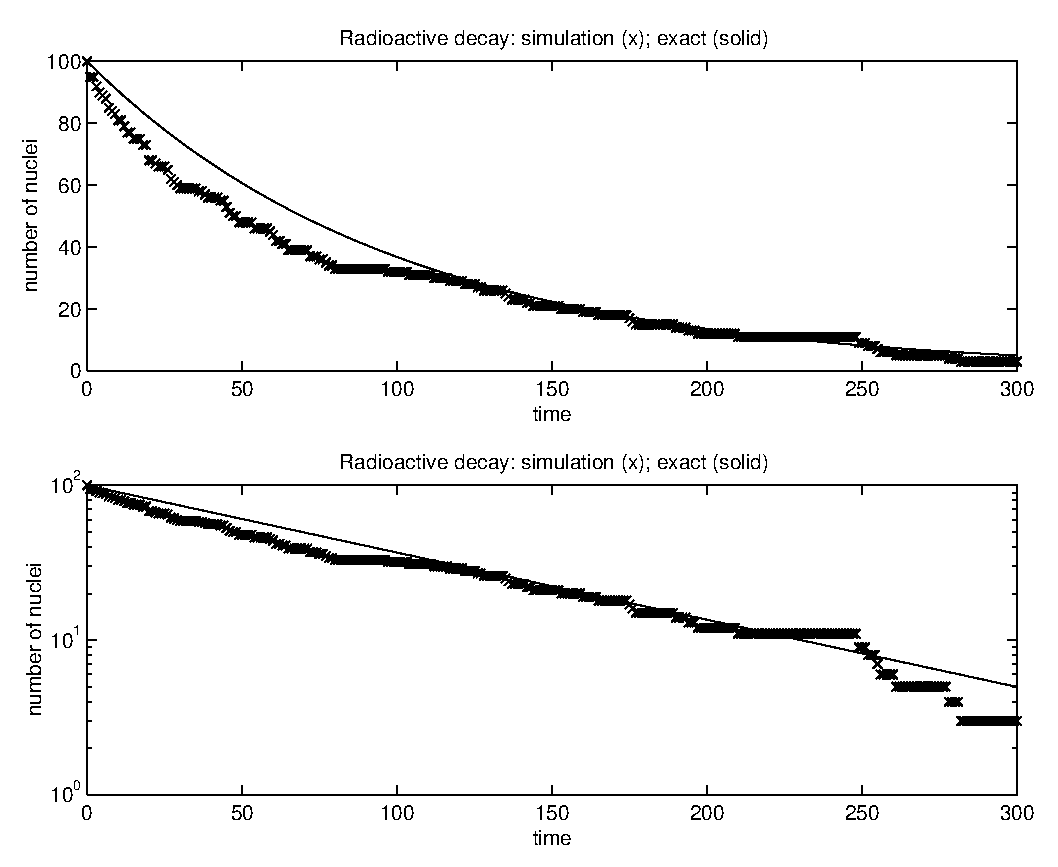
\includegraphics[width=10cm]{f_decaya.eps}
\caption{A realization of the stochastic process of radioactive decay.
The parameters of the simulation were $N_0 = 100; 
\quad p = 0.01 s^{-1}; \quad \Delta t = 1s;  \quad tend = 300s$}
\end{figure}
\begin{figure}
\label{FIG_DECAYB}
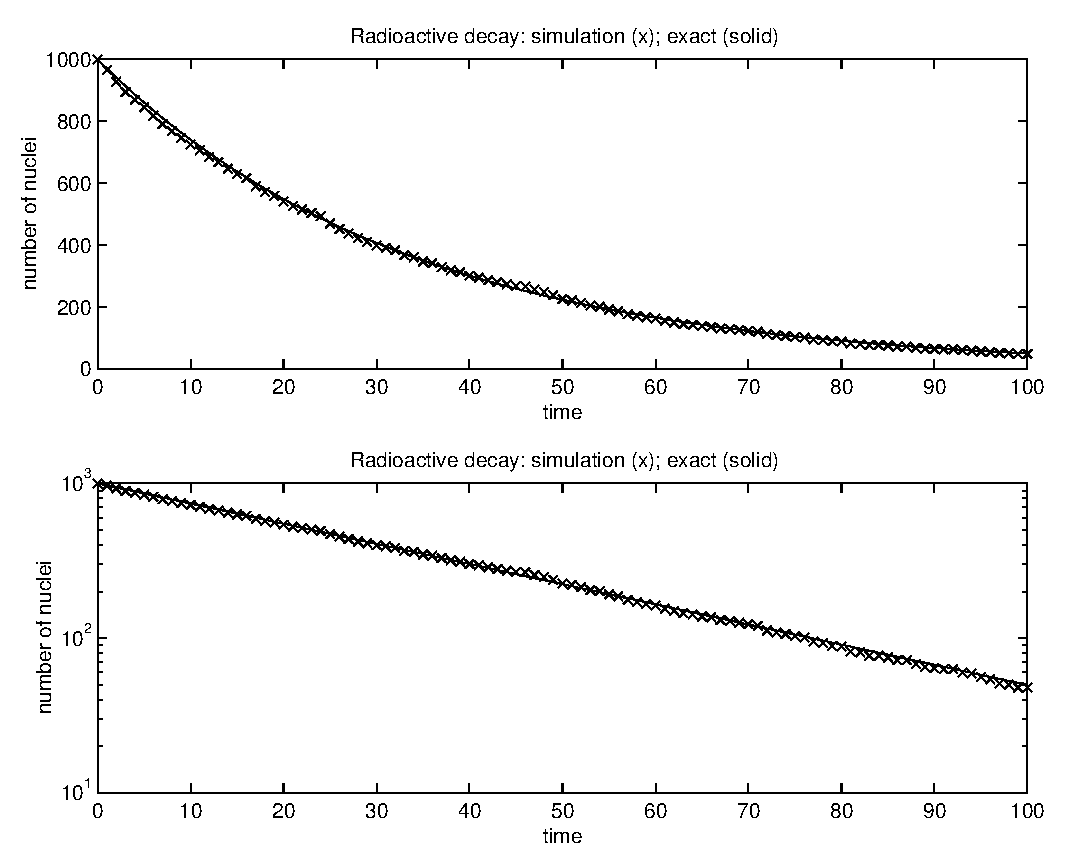
\includegraphics[width=10cm]{f_decayb.eps}
\caption{A realization of the stochastic process of radioactive decay.
The parameters of the simulation were $N_0 = 1000; 
\quad p = 0.03 s^{-1}; \quad \Delta t = 1s;  \quad tend = 100s$}
\end{figure}
 It is 
immediately recognized that the simulation results fluctuate around 
the expected curve. This is of course not astonishing since the 
exact result holds for mean values. In order to achieve a better
agreement with the decay law it is necessary to run the simulation
several times and to take the average over the different 
realizations of the decay process. This can easily be achieved by 
a simple modification of the program {\sf decay}. We 
introduce an additional input variable, the number of realizations
{\sf nreal} and accordingly implement a loop over the different 
realizations. This can be best seen in the listing of the 
new program {\sf decayr}.


At the end of the realizations loop
we have to perform the average. This is seen in lines xy.
(STRESS MORE THE IDEA OF REALIZATIONS!!!!; allgemeine Strategie erlaeutern.)

Note that in order to speed up the program we have modified slightly 
the algorithm  so that we can save a loop.
The probability to observe one decay in time $\Delta t$ is
\begin{equation}
p = \beta \Delta t
\end{equation}
where $\beta = \lambda N$ and $\Delta t$ must be small enough so 
that $\beta \delta t \ll 1$. 
From the elementary rules of combinatorics we know that
the probability to observe $n$ decays in time $t=m\Delta t$ is therefore
given by
\begin{equation}
P = p^n(1-p)^{m-n} {m \choose n}.
\end{equation}
Inserting the definition of $p$ the above expression can be cast 
in the form
\begin{equation}
P = \left( \frac{\beta t}{m}\right)^n 
     \left( \frac{1 - \beta t}{m} \right)^{m-n}
      \frac{m!}{(m-n)! n!}.
\end{equation}
Performing the limit $\Delta t \longrightarrow 0$ (i.e. $m 
\longrightarrow \infty$) and considering that
\begin{equation}
\left(1-  \frac{\beta t}{m} \right)^{m} \longrightarrow 
            \exp(-\beta t),
\end{equation}
\begin{equation}
\left( 1- \frac{ \beta t}{m} \right)^{-n} \longrightarrow 
            1,
\end{equation}
and
\begin{equation}
\frac{m!}{(m-n)! n!} \longrightarrow m^n
\end{equation}
we obtain the result
\begin{equation}
P = \frac{\mu^n \exp(-\mu)}{n!},
\end{equation}
where $\mu = \beta t$. The above distribution is the well know
Poisson distribution.

It is now easy to verify that the number of decays in a given 
interval is distributed according to the Poisson distribution.
To this end we have counted the number of decays in a given 
interval. This is accomplished in the lines xy. At the end of the
program we plot in a histogram the distribution of the number of 
decays and overlay the expected Poisson
distribution.  This is achieved in the program {\sf decayr} with the 
help of the {\sf hold} command. When you set "{\sf hold on}" MATLAB does not 
remove the existing graph; the following data are addeded to the 
current graph. The overplotting of data is terminated by 
setting "{\sf hold off}".

\subsubsection{Listing of the program decayr}
\inputlisting{./Listings/decayr.m}


Run the program for the following two sets of parameters:
\begin{eqnarray*}
N_0= 100, p = 0.001 s^{-1}, \Delta t = 1s, t = 100s \\
N_0= 100, p = 0.0001 s^{-1}, \Delta t = 1s, t = 100s
\end{eqnarray*}
with nreal = 100 and nreal = 1000.

The result of  two simulations can be seen in figs. x and y.
\begin{figure}
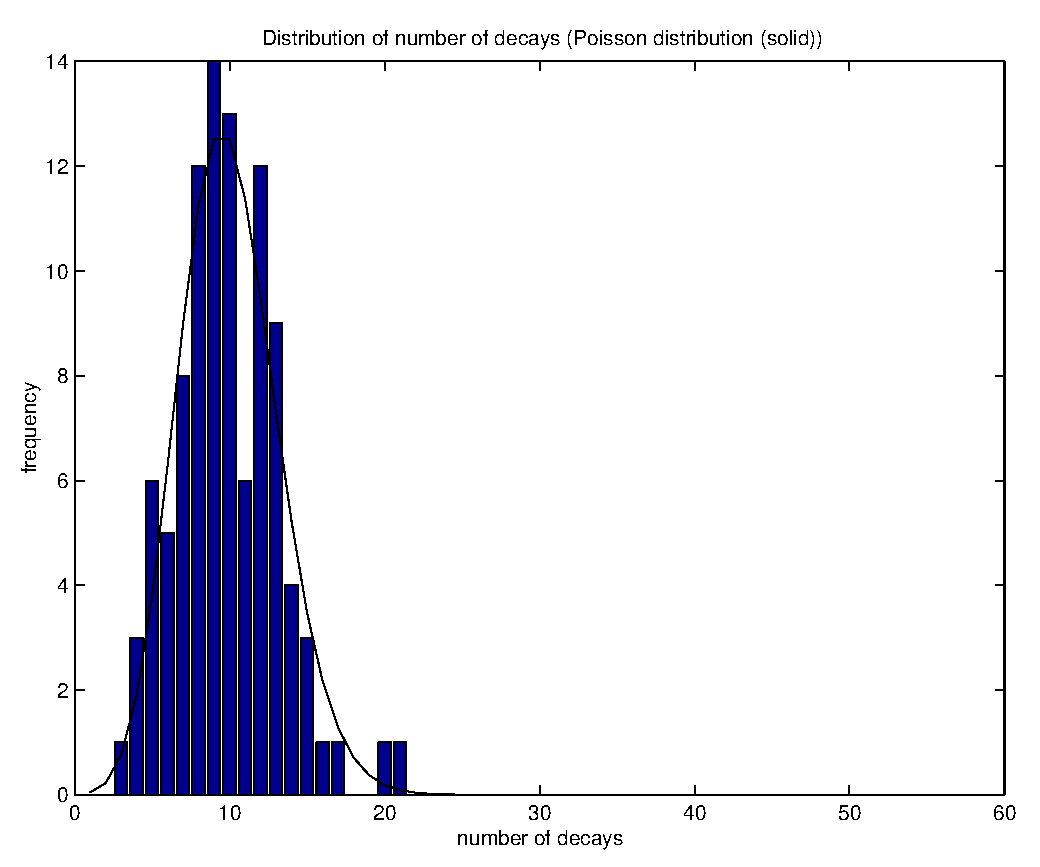
\includegraphics[width=\textwidth]{f_decay1.eps}
\caption{The distribution of the number of decays computed with 
the program decayr. 100 realizations. The simulation was run for
N0=100 and lambda=0.001.}
\end{figure}

\begin{figure}
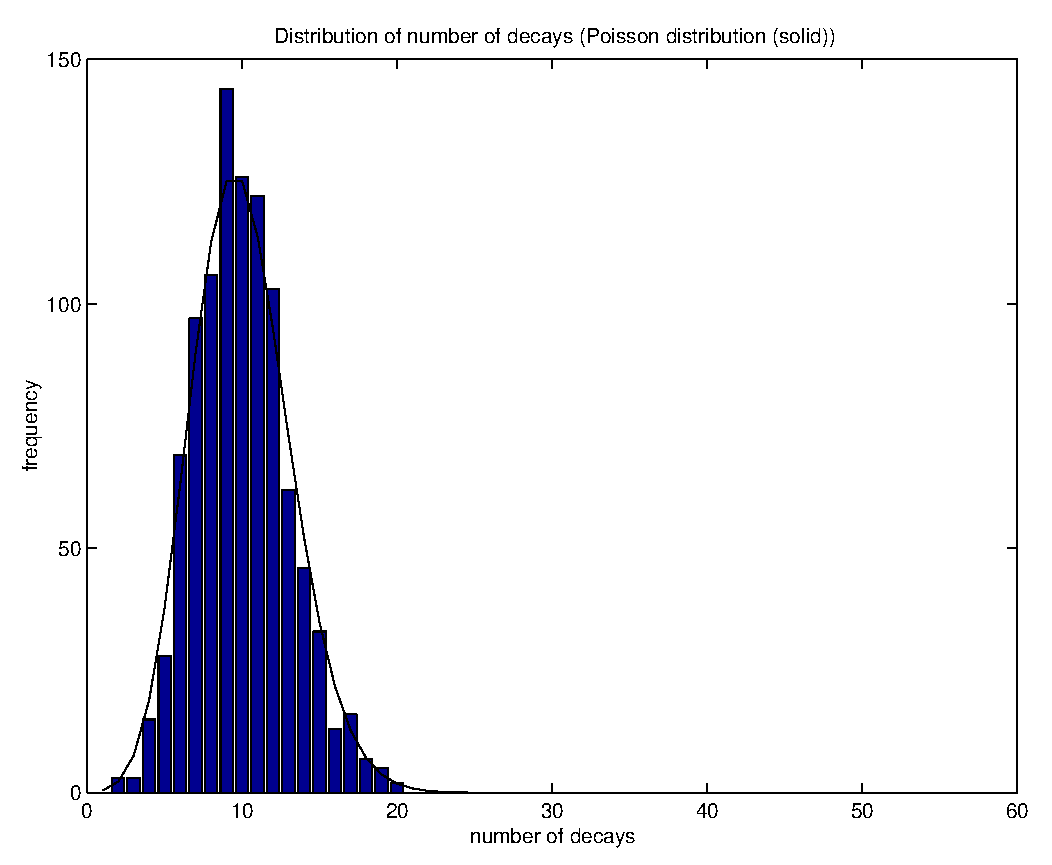
\includegraphics[width=\textwidth]{f_decay2.eps}
\caption{The distribution of the number of decays computed with 
the program decayr. 1000 realizations. The simulation was run
for N0=100 and lambda = 0.001.}
\end{figure}

%%%%%%%%%%%%%%%%%%%%%%%%%%%%%%%%%%%%%%%%%%%%%%%%%%%%%%%%%%%%%%%%%%%%%%
\section{Simple Monte Carlo evaluation of integrals}
It is the purpose of this subsection to introduce Monte Carlo Methods
in the context of the numerical evaluation of definite integrals.
We will see in later chapters that Monte Carlo integration is the
method of choice when treating multidimensional
integrals numerically. As a typical rule of thumb
``classical'' deterministic methods are outperformed
by Monte Carlo methods  for systems with a large number of 
degrees of freedom.
For simplicity and to stress the basic ideas 
it is convenient at the moment to consider one--dimensional definite
integrals of the form
\begin{equation}
\label{INTEGRAL}
I = \int_a^b dx f(x).
\end{equation}
Obviously such integrals can be evaluated analytically for many
integrands
$f(x)$.  However, there are as well many cases for which a numerical
evaluation is necessary.

Before introducing the Monte Carlo approach to numerical integration
let us remind the basic ``classical'' deterministic approach to
numerical integration. The standard approach is based upon the
geometrical interpretation of the integral (\ref{INTEGRAL}) as the
area under the curve of the function $f(x)$ between the points $a$ and
$b$. In the simplest algorithm this area (see figure) is approximated
as a sum over rectangles. To this end the $x$--axis is divided into
$n$ equally spaced intervals of width $\Delta x$,
\begin{equation}
\Delta x = \frac{b-a}{n}
\end{equation}
whose ends are given by
\begin{equation}
x_i = x_0 + i\Delta x
\end{equation}
for $i=1, \ldots ,n$. Of course, $x_0 = a$ and $x_n =b$. Thus in the
so--called rectangular approximation the integral is evaluated as
\begin{equation}
\label{I_CLASSICAL}
I_n = \Delta x \sum_{i=0}^{n-1} f(x_i).
\end{equation}
Of course, other more accurate approximations are possible.

How can we now evaluate the above integral by drawing random numbers?
The standard way is based on a very simple idea. 
From the introductory course in analysis we know that the Mean 
Value Theorem states that the exact value of the integral $I$ is 
given by
\begin{equation}
I= (b-a) f(\zeta)
\end{equation}
for some value of $\zeta$ in the interval $a \le \zeta \le b$. $f(\zeta)$
represents the average value of the function $f(x)$ 
in the interval $[a,b]$. Thus we could also write
\begin{equation}
I = (b-a) \langle f \rangle,
\end{equation}
where $\langle  \rangle$ denotes the mean value.
Let us draw $n$
random numbers which are uniformly distributed in the interval $[a,b]$
and let us sample the corresponding value of $f(x_i)=f_i$. The Monte Carlo
estimate $I_n$ of the integral $I$ is then the sample mean, which is
given by
\begin{equation}
\label{MCI_STANDARD}
I_n = \frac{(b-a)}{n} \sum_{i=1}^{n} f(x_i),
\end{equation}
where $n$ is the number of trials. Amazingly the form of the above
estimate is very similar to the classical formula (\ref{I_CLASSICAL}).
The fundamental difference is that now the $n$ points at which the
function $f$ is evaluated are no longer equally spaced but randomly 
distributed.

There is also the possibility to compute the integral $I$
stochastically
with the help of the ``Hit or Miss'' algorithm. The idea behind
this algorithm is again very simple. To be explicit we imagine a rectangle
of height $h$ and width $(b-a)$ such that the function $f(x)$ lies
within the rectangle (see figure; Gould, p.329). To evaluate the
integral we draw randomly pairs of uniformly distributed random
numbers $(x_i,y_i)$ such that $a \le x_i \le b$ and $0 \le y_i \le h$.
In other words the probability to draw a point within the rectangle is
given by the inverse of the area $A$ of the rectangle,
i.e. $1/(b-a)h$. It is now evident how the area under the
function $f$ may be estimated. The fraction of points $(x_i,y_i)$
which satisfy the condition $y_i \le f(x_i)$ is an estimate of the
ratio of the integral $I$ to the area $A$ of the rectangle. Hence,
drawing $n$ random pairs the estimate $I_n$ of $I$ by this ``scoring''
method is given by
\begin{equation}
I_n = A \frac{n_s}{n},
\end{equation}
where $n_s$ is the number of ``hits'', i.e., of points lying below the
curve $f(x)$.

Before writing two simple programs to elucidate the above algorithms
it is important to have in mind that both estimates are affected by
statistical errors. Let us consider for simplicity 
the standard method. Since the $f(x_i)$ are random we know 
from the elementary theory of data analysis
that an appropriate measure of the error is given by the variance
which is defined by
\begin{equation}
{\rm Var}(f) = \langle f^2 \rangle - \langle f \rangle^2.
= \langle (f -\langle f \rangle)^2 \rangle
\end{equation}
Since we draw a finite number of random numbers we can
estimate the mean value by using
\begin{equation}
\hat{f}  = \frac{1}{n} \sum_{i=1}^n f(x_i) 
\end{equation}
and correspondingly the estimate of the variance by using
\begin{equation}
{\rm Var}(f(x_1),\ldots, f(x_n)) = \frac{1}{n-1} \sum_{i=1}^n 
   (f(x_i)- \hat{f})^2 = \sigma_f^2.
\end{equation}
The quantity $\sigma_f = \sqrt{{\rm Var}(f_1, \ldots, f_n)}$ 
is also called the standard deviation. In the previous expression
we have used the short--hand
notation $f(x_i) = f_i$. However,
we are not interested in the error of $f$ but in the error of the
estimate $I_n$ which is a sum over random numbers. 

Repeating the 
simulation and hence drawing other random numbers we will get another
estimate of $I_n$. Therefore, repeating the simulation $m$ times 
we can estimate the mean of $I_n$ as
\begin{equation}
\hat{I_n} = \frac{1}{m} \sum_j^m I_n(j)
\end{equation}
and the corresponding variance as
\begin{equation}
{\rm Var}(I_n(1), \ldots, I_n(m)) = 
\frac{1}{m-1} \sum_j^m (I_n(j) - \hat{I_n})^2 = \sigma_I^2
\end{equation}
We will denote the above variance also by $\sigma_I^2$.
Of course, proceeding this way is not very practical since we
have to perform the simulation $m$ times. A much more economical
estimation of the error of the mean of $I_n$ could be achieved by 
establishing a simple relation between $\sigma_I$ and the standard 
deviation of the individual trials $\sigma_f$. To this end we 
introduce the discrepancy $\delta f_i$ between the
individual trial $f_i$ and its mean $\langle f \rangle$. The 
discrepancy $\delta I_n$ between $I_n$ and its mean value can be
obtained to first order in the $\delta f_i$ by a simple Taylor 
expansion (error propagation rules)
\begin{equation}
\delta I_n = \sum_{i=1}^n \frac{\partial I_n}{\partial f_i} \delta 
f_i.
\end{equation}
Hence, it follows from the above equation by taking the average over
$\delta I_n^2$ that
\begin{equation}
\langle \delta I_n^2 \rangle = \sum_{i,j=1}^{n}
    \frac{\partial^2 I_n}{\partial f_i \partial f_j} 
     \langle \delta f_i \delta f_j \rangle.
\end{equation}
It is plausible to assume, that 
$\langle \delta f_i \rangle = 0$
for all $i$ and that the $\delta f_i$ are not correlated
for $i \neq j$, i.e.,
$\langle \delta f_i \delta f_j \rangle = \langle f_i \rangle \langle f_j \rangle$
and that for $i=j$ we have $\langle \delta f_i^2 \rangle = \sigma_f$ 
for all $i$ it follows from the above equation that
\begin{equation}
\sigma_I^2 = \sum_{i=1}^n \left(
      \frac{\partial I_n}{\partial f_i} \right)^2 \sigma_f^2
      = \frac{1}{n^2} n \sigma_f^2 = \frac{\sigma_f^2}{n}
\end{equation}
and finally we have the useful relation
\begin{equation}
\sigma_I = \frac{\sigma_f}{\sqrt{n}}.
\end{equation}
The mean error of the mean scale with 1 over the square root of 
the number of individual trials. The precision of the estimate 
thus increases only slowly with the number of trials (remark: central
limit theorem: see Chapter 2).

Now we are in the position to write two programs to implement the above
stochastic algorithms. In order to be specific we compute the integral
\begin{equation}
I = \int_0^1 dx \sqrt{1-x^2} = \frac{\pi}{4}.
\end{equation}
In other words we want to estimate the number $\pi$ by Monte Carlo
methods.

We begin by the standard method. The listing of an according 
program can be seen below.

\subsubsection{Listing of the program mcpi.}
\inputlisting{./Listings/mcpi.m}

We run the program for $n=10, 100, 1000, 10000$. The result of the 
four simulations can be seen in Fig. xy.
\begin{figure}
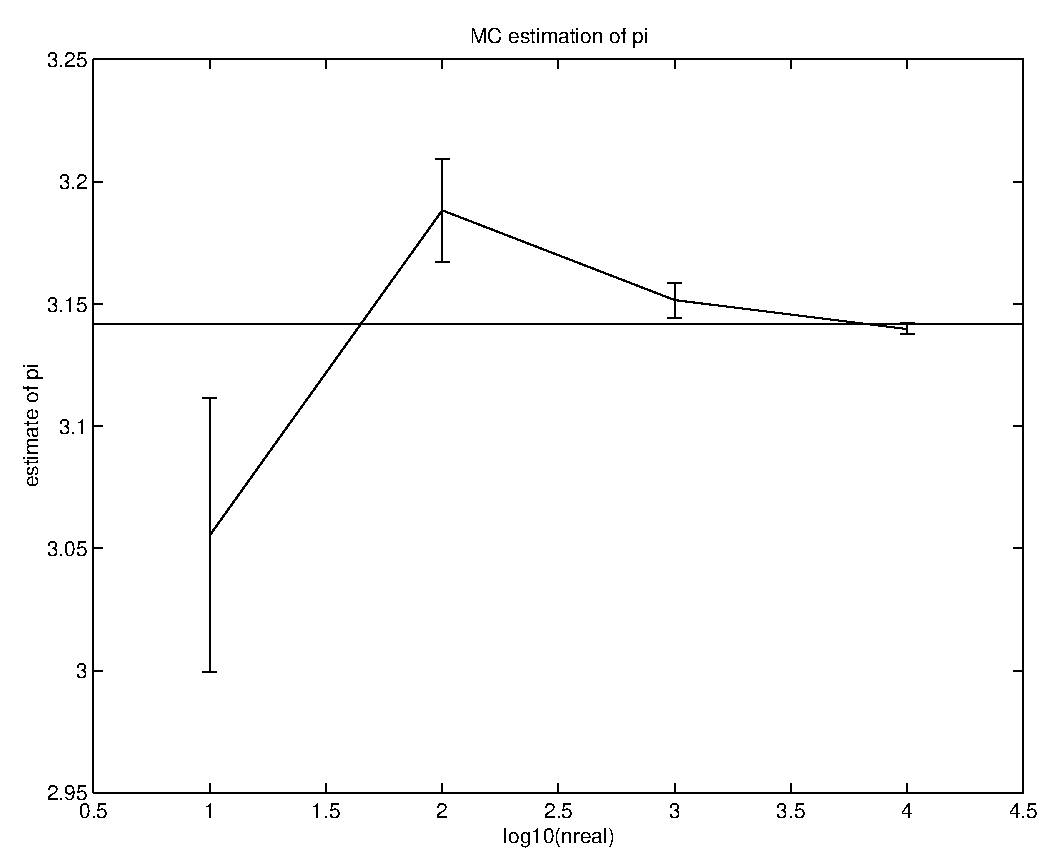
\includegraphics[width=\textwidth]{plotmcpi.eps}
\caption{The estimation of pi for n=10,100,1000,10000. The 
error bars correspond to the standard deviation of the mean of the 
estimate.}
\end{figure}

Next we write a program for the scoring  method. 

\subsubsection{Listing of the program mcpiscore.m}
\inputlisting{./Listings/mcpiscore.m}

Again we run the simulation for n=10, 100, 1000, 10000.
The result of a simulation can be seen in the next Figure.
\begin{figure}
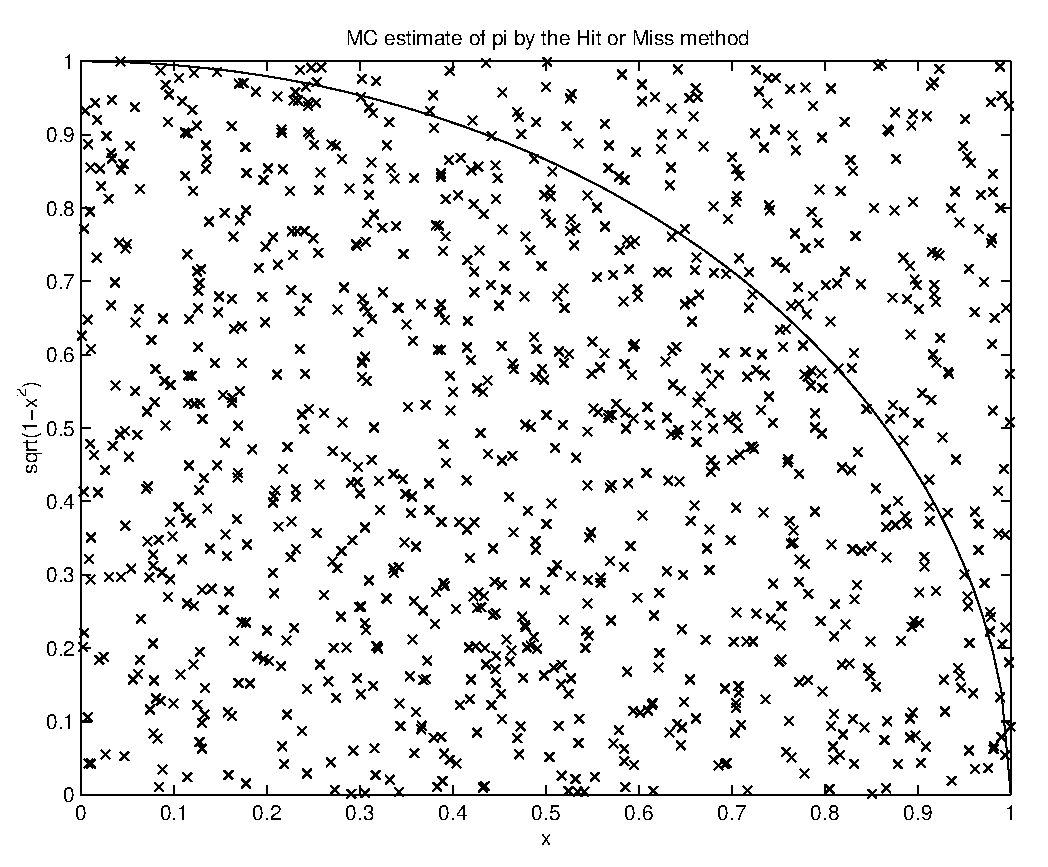
\includegraphics[width=\textwidth]{fmcpiscore.eps}
\caption{The scoring method. The continuous line represents
the function $\sqrt{(1-x^2)}$.}
\end{figure}


%%%%%%%%%%%%%%%%%%%%%%%%%%%%%%%%%%%%%%%%%%%%%%%%%%%%%%%%%%%%%%%%
\section{Beyond this chapter}


%%%%%%%%%%%%%%%%%%%%%%%%%%%%%%%%%%%%%%%%%%%%%%%%%%%%%%%%%%%%%%%%
\section{Exercises}
{\bf Exercise 1.} Write a program to simulate photoabsorption.
    Lit. Whitney

{\bf Exercise 2.} Write a program for the Monte Carlo estimation of
the following integral
\begin{equation}
\int_0^1\frac{dx}{1+x^2} = \frac{\pi}{4}
\end{equation}

{\bf Exercise 3.} Write a program to evaluate the number $e$ by a
stochastic method.
Lit: Pirooz Mohazzabi, Monte Carlo estimation of $e$,
Am. J. Phys. {\bf 66} (1998) 138--140.


\bibliographystyle{peter}
\bibliography{V_98}
